
\begin{frame}{ElGamal Run ratio Experiment}
    If we consider $\rho(t)$ as the occurrences of all runs of length $t$, we expect that 
    $$ \rho(t+1)/\rho(t) = \frac{1}{v} $$
    from Golomb's postulates of randomness.
\end{frame}

\begin{frame}{ElGamal Sequences run ratio Experiment}
    \begin{columns}
        \begin{column}{0.45\textwidth}
            \begin{figure}
                \centering
                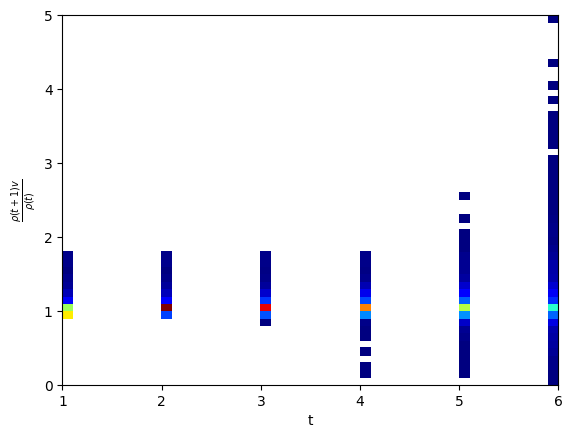
\includegraphics[width=\textwidth]{figures/AllDataNormalizedrunratio.png}
                \caption{Distribution of $\rho(t+1)v/\rho(t)$ as a heatmap}
            \end{figure}
        \end{column}
        \begin{column}{0.45\textwidth}
            \begin{figure}
                \centering
                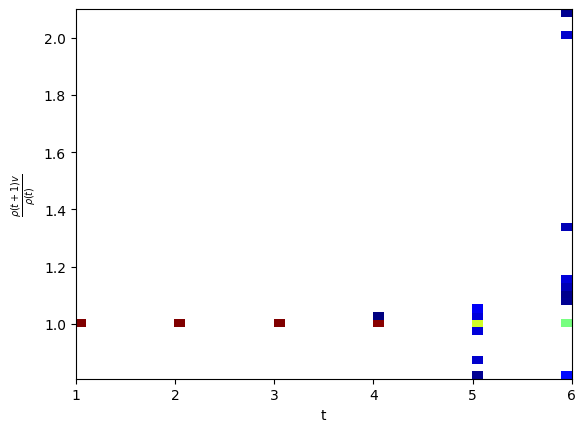
\includegraphics[width=\textwidth]{figures/AllDataAndvisGenNormalizedrunratio.png}
                \caption{Distribution of $\rho(t+1)v/\rho(t)$ with $v = g$ as a heatmap}
            \end{figure}
        \end{column}
    \end{columns}
\end{frame}

\begin{frame}{ElGamal Sequences run ratio Experiment}
    \begin{columns}
        \begin{column}{0.45\textwidth}
            \begin{figure}
                \centering
                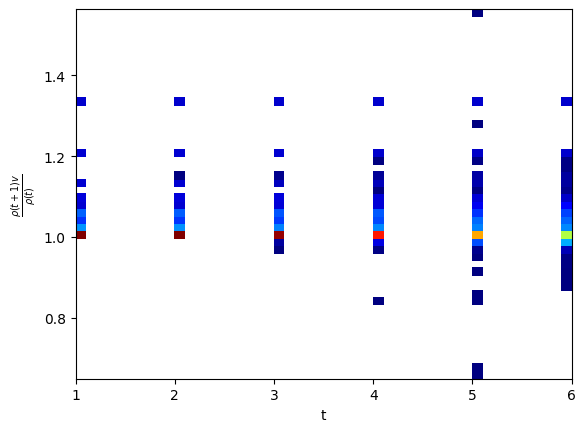
\includegraphics[width=\textwidth]{figures/v2Normalizedrunratio.png}
                \caption{Distribution of $\rho(t+1)v/\rho(t)$ and $v = 2$ as a heatmap}
            \end{figure}
        \end{column}
        \begin{column}{0.45\textwidth}
            \begin{figure}
                \centering
                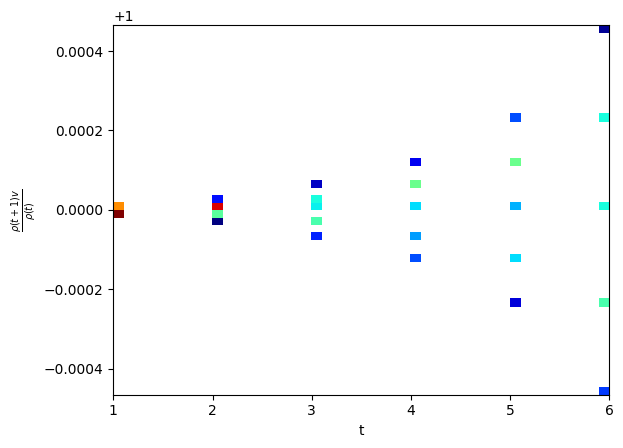
\includegraphics[width=\textwidth]{figures/v2AndvisGenNormalizedrunratio.png}
                \caption{Distribution of $\rho(t+1)v/\rho(t)$ with $v = g = 2$ as a heatmap}
            \end{figure}
        \end{column}
    \end{columns}
\end{frame}

 	

%%% Local Variables:
%%% TeX-master: "../main.tex"
%%% End:
